\section{gyakorlat (2025. november 5.)}
\subsubsection*{"Hasonló" feladatok}

\subsubsection*{1. Rúd szétvágása}
Adott egy $l$ hosszúságú rúd, amit $l_1, l_2, \cdots, l_n$ hosszú darabokra akarunk felvágni, adott vágási pontoknál.

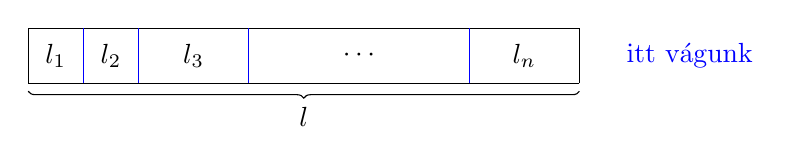
\begin{tikzpicture}[scale=0.7]
\draw (0,0) -- (10,0);
\draw (0,1) -- (10,1);

\draw (0,0) -- (0,1);
\draw[blue] (1,0) -- (1,1);
\draw[blue] (2,0) -- (2,1);
\draw[blue] (4,0) -- (4,1);
\draw[blue] (8,0) -- (8,1);
\draw (10,0) -- (10,1);

\node at (0.5,0.5) {$l_1$};
\node at (1.5,0.5) {$l_2$};
\node at (3,0.5) {$l_3$};
\node at (6,0.5) {$\cdots$};
\node at (9,0.5) {$l_n$};

\draw[decoration={mirror, brace, raise=0.1cm}, decorate] (0,0) -- (10,0);

\node at (5, -0.6) {$l$};
\node[blue] at (12, 0.5) {itt vágunk};
\end{tikzpicture}


Egy vágás úgy zajlik, hogy a már korábban "levágott" darabok valamelyikét felemeljük a vágóeszközre, és az ottani vágási pontok valamelyikén vágunk.
Egy ilyen vágás költsége legyen az épp vágott darab részeinek összege.

\textbf{Példa:}

\includegraphics[width=7cm]{gy/img/gy08_cut_step_1}\\
\textbf{1. vágás} (költség: 18)

\includegraphics[width=7cm]{gy/img/gy08_cut_step_2}\\
\textbf{2. vágás} (költség: 11)

\includegraphics[width=7cm]{gy/img/gy08_cut_step_3}\\
\textbf{3. vágás} (költség: 7)

\includegraphics[width=7cm]{gy/img/gy08_cut_step_4}\\
\textbf{4. vágás} (költség: 7)

\includegraphics[width=7cm]{gy/img/gy08_cut_step_5}\\
\textbf{5. vágás} (költség: 4)

\includegraphics[width=7cm]{gy/img/gy08_cut_step_6}\\
\textbf{6. vágás} (költség: 5)

\includegraphics[width=7cm]{gy/img/gy08_cut_step_7}

\textbf{Költség összesen:} 52

Van ennél kisebb összköltségű vágássorozat?
Mi a legkisebb összköltség?

Vegyük észre az analógiát az optimális zárójelezés feladattal!
Várhatóan DP egy alkalmas módszer lesz a megoldásra, analóg módon a zárójelezéshez.

(margó szélére: ha $n$ darabra vágunk, összesen $(n-1)!$ lehetőség van erre, persze ezek közül nem mind "lényegesen különböző")

Részproblémák \rightarrow "infixek optimális szétvágása"

\textbf{HF.} részletek kidolgozása

\textbf{Változat:} a vágási pontokat is nekünk kell meghatározni (persze $l = l_1 + l_2 + \cdots + l_n$ továbbra is).
A példát tekintve itt megengedett első vágásnak a bal szélről levágni egy 4 hosszú darabot.

Érdemes visszafelé elképzelni a vágássorozatot ("ragasztások sorozata").

Példánkban:
\nopagebreak

\includegraphics[width=8cm]{gy/img/gy08_cut_reverse}

Mohó heurisztika: mindig a két legrövidebb darabot ragasztjuk összeadjuk
Bizonyítani kell, hogy ezek a lokálisan optimális lépések elvezetnek a globális optimumhoz.

Nagyon hatékony $\rightarrow$ kupaccal $\mathcal{O}(n \log n)$ lépés (eredeti változat DP-vel $\rightarrow \mathcal{O}(n^3)$).

Nagyon hasonló ez az egész az információtömörítésnél megismert Huffman algoritmushoz (Huffman-kódhoz).

\subsubsection*{2. Optimális bináris keresőfa}
Általában bináris keresőfákat dinamikusan változó adathalmazokra alkalmazunk.
Itt most statikus lesz az adathalmaz ezzel szemben.
Itt ismert az adatelemek keresési gyakorisága is.
Olyan bináris keresőfa megépítése a cél az adatelemekből, ahol a keresési út hosszának várható értéke minimális.